\begin{frame}[fragile]
\frametitle{Optimierung von $K$}

\begin{itemize}
  \item Bestimmung von $K$ mit linear vorverzerrten Signal
  \item Anpassung von $K$ für nichtliniear vorverzerrte Signale
\end{itemize}

\begin{align}
	U_{?, \mathrm{meas}} (t) = \sum_{n=1}^N \, \overline{a}_n \left[ U_{in}(t)\right]^n
	\quad
	U_{?, \mathrm{ideal}} (t) = \sum_{n=1}^N \, a_n \left[ U_{in}(t) \right]^n
\end{align}
\begin{itemize}
  \item Oder direkt über die Differenz der Signale
\end{itemize}
\begin{align}
	\Delta U_? (t) = U_{?, \mathrm{meas}} (t) - U_{?, \mathrm{ideal}} (t)
	=
	\sum_{n=1}^N \, \left( \overline{a}_n -  a_n\right) \left[ U_{in}(t) \right]^n
	=
	\sum_{n=1}^N \, \tilde{a}_n \, \left[ U_{in}(t) \right]^n
\end{align}
\end{frame}

\begin{frame}[fragile]
\frametitle{Optimierung von $K$}
\begin{itemize}
	\item Bestimmung der Parameter $\tilde{a}_n$
	\item Vergleichen der Samples ${\Delta U_{?,i} = \Delta U_? (i \cdot \Delta t)}$ mit ${U_{in,i} = U_{in}(i \cdot \Delta t)}$
	\item Lösung des linearen Optimierungsproblems ergibt die Anpassung der alten Parameter
\end{itemize}
\begin{align}
	a_n^{i+1} = a_n^{i} + \sigma_{a}^{i} \tilde{a}_n^{i}
\end{align}
	
\end{frame}

\begin{frame}
\frametitle{Erster Ansatz}
\begin{picture}(10,7)
		\put(0,-160){
			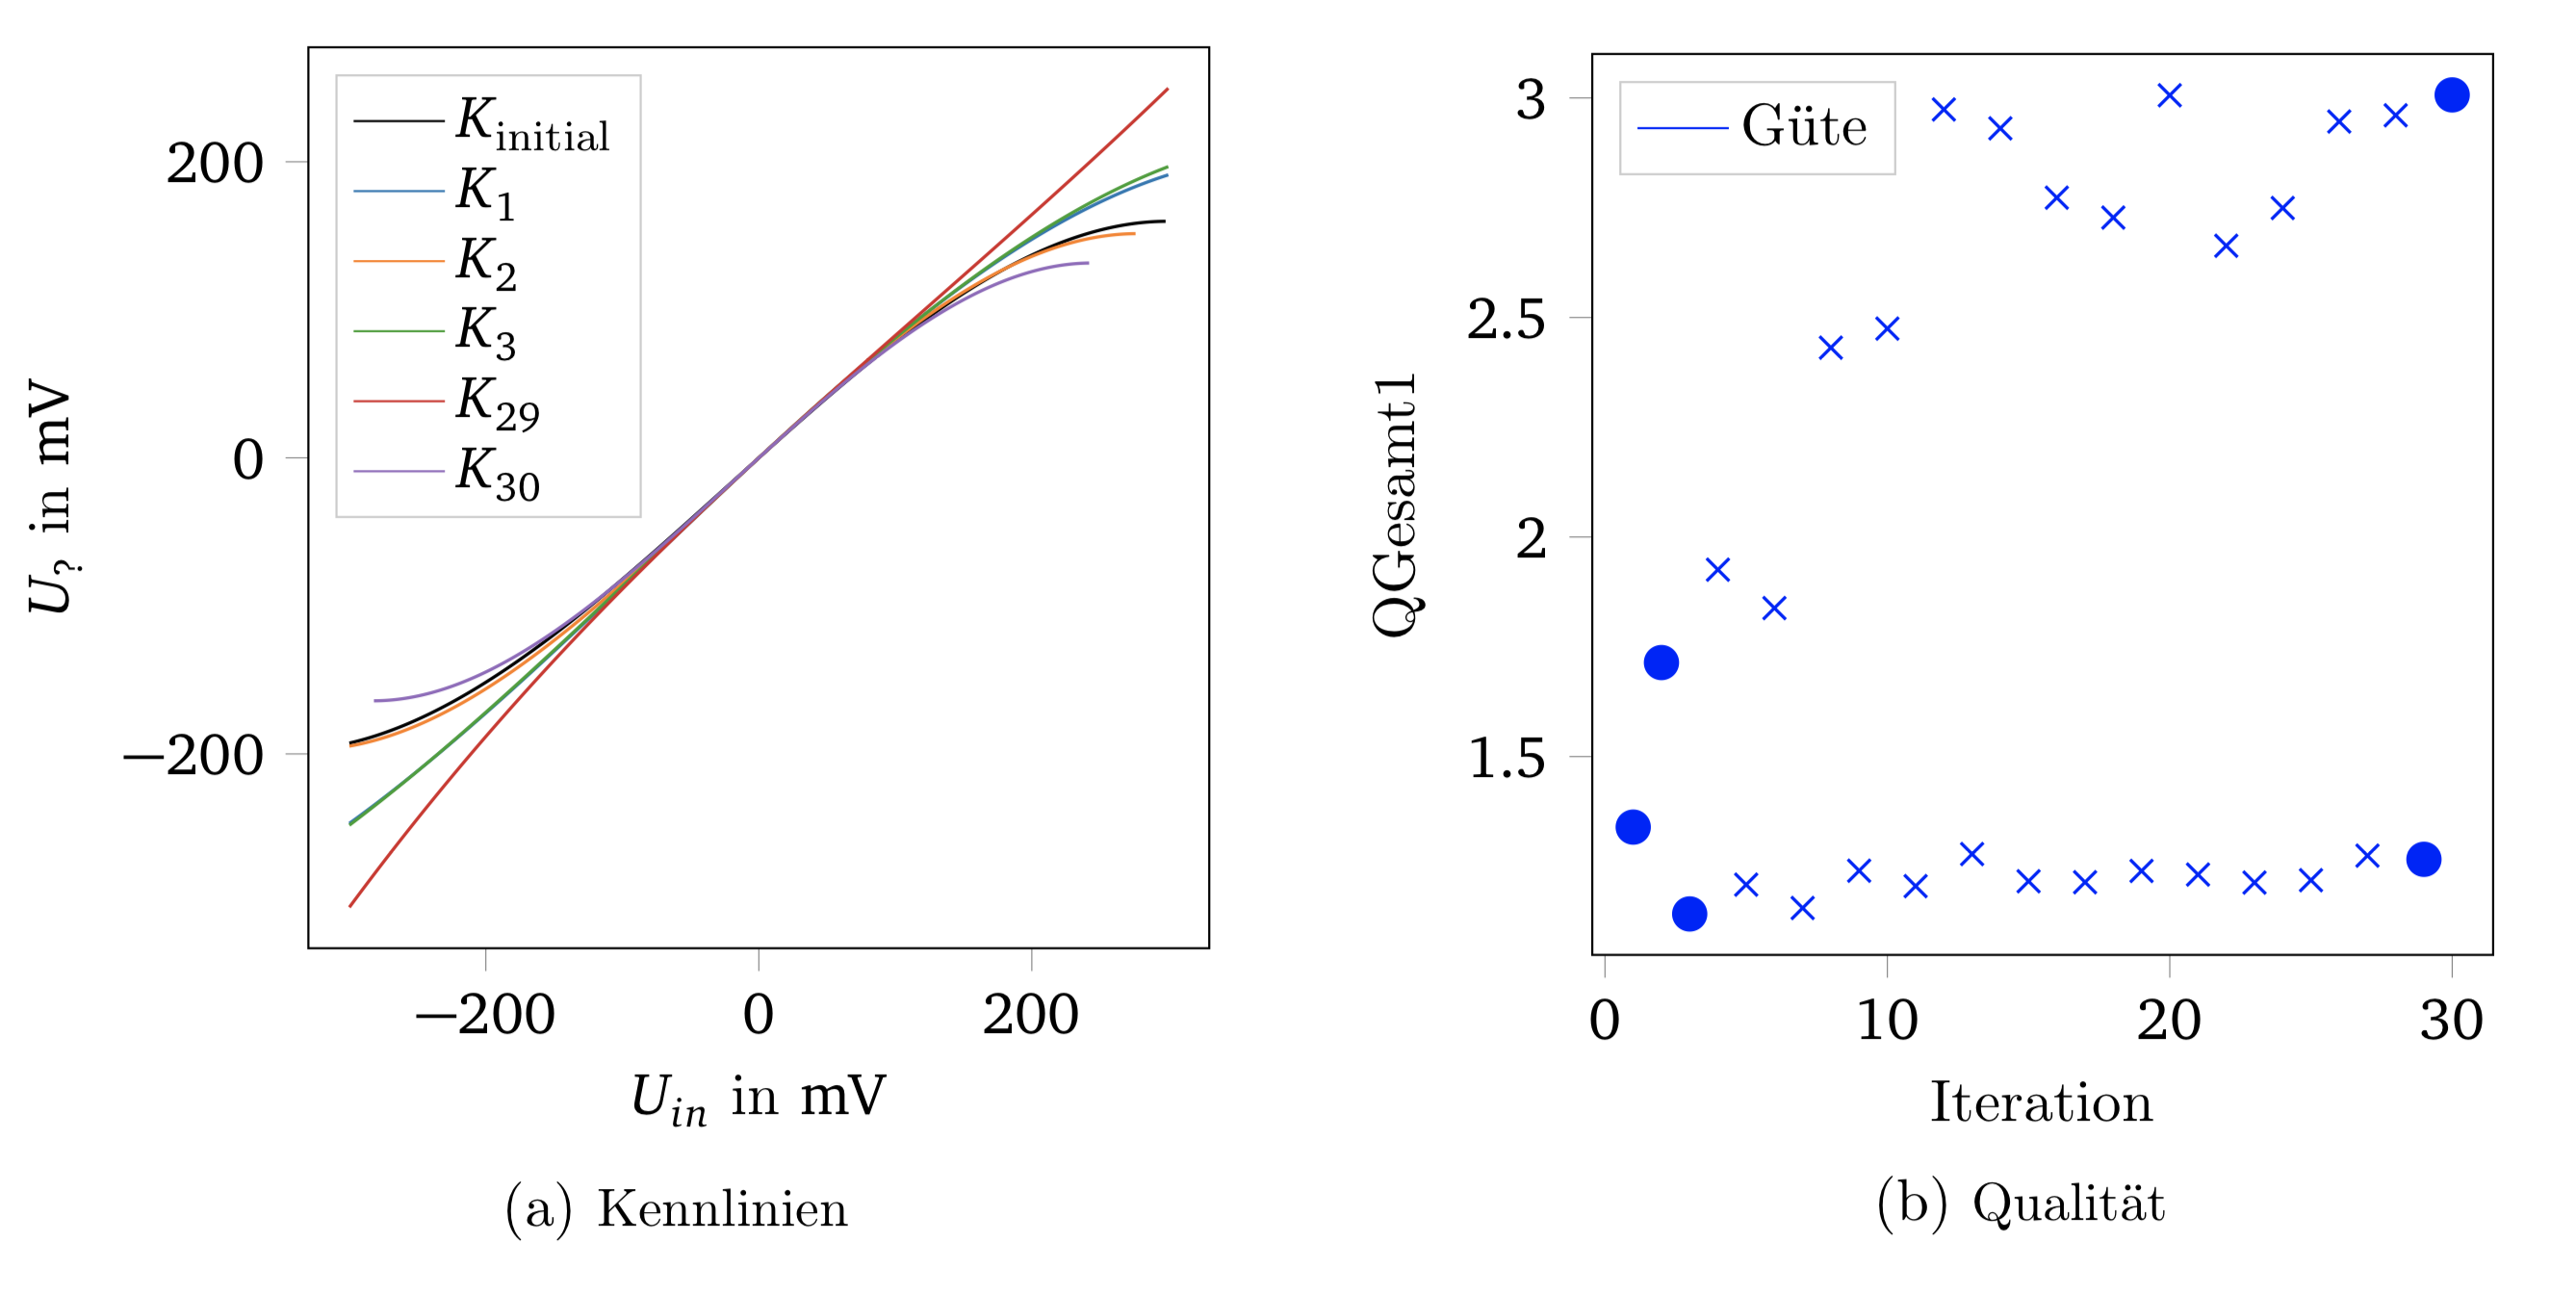
\includegraphics[scale=0.25]{slides/adjust_a/30Iteration.png} 
		}  
	\end{picture}
\end{frame}
